% LTeX: language=de-DE
\chapter{Evaluation}
	Im Folgenden sollen die mechanische Integrität und Performance des Systems mit Respekt auf die in \cref{sec:constructive limitations} formulierten Rahmenbedingenungen diskutiert werden.
	Im Vorfeld wurden mehrere Testfahrten auf urbanem Untergrund Untergrund und entlang verschiedener Steigungen durchgeführt.
	Zurückgelegte Distanz und mittlere, sowie maximale Geschwindigkeit wurden mittels Navigationssoftware und GPS gemessen.
	Da aus Sicherheitsgründen einige Testläufe auf der Werkbank durchgeführt wurden, Messungen per GPS jedoch eine tatsächliche Bewegung im freien zwingend erforderlich machen wurden zusätzlich Logginginformationen der ESC ausgelesen um aus Umdrehungen pro Minute und Anzahl der Umdrehungen die gleichen Informationen ermitteln zu können.\par\medskip
	%
	\Cref{fig:real world assembly} zeigt den Gesamtaufbau des Systems mit zwei Motoren, den Unterbaugruppen der Motorhalterungen, den Riemen, die Rollen und den hinteren Truck.
	Von den Riemen verdeckt an den Rollen befinden sich die Zahnscheiben.
	\begin{figure}[h]
		\centering
		\includegraphics[angle=180, width=.8\textwidth]{Footage/Pictures/Drivetrain close up v2.jpg}
		\caption[Fertiger Aufbau des Antriebssystems]{Fertiger Aufbau des Antriebssystems nach etwa \qty{50}{\kilo\metre} Testfahrt durch urbanes Terrain.}
		\label{fig:real world assembly}
	\end{figure}

	\section{Performance}
		Im Leerlauf wurde zunächst auf der Werkbank die tatsächliche Maximalgeschwindigkeit mit der theoretischen verglichen.

	\begin{figure}[h]
		\centering
		\subcaptionbox{Ungenutzte Druckteile.\label{subfig:freshly printed pulleys}}[.49\textwidth][l]{
			\includegraphics[angle=180, width=.49\textwidth]{Footage/Pictures/Wheel pulley v2.jpg}
		}
		\subcaptionbox{Zustand der Druckteile nach einigen Testfahrten.\label{ubfig:printed pulleys after test driving}}[.49\textwidth][r]{
			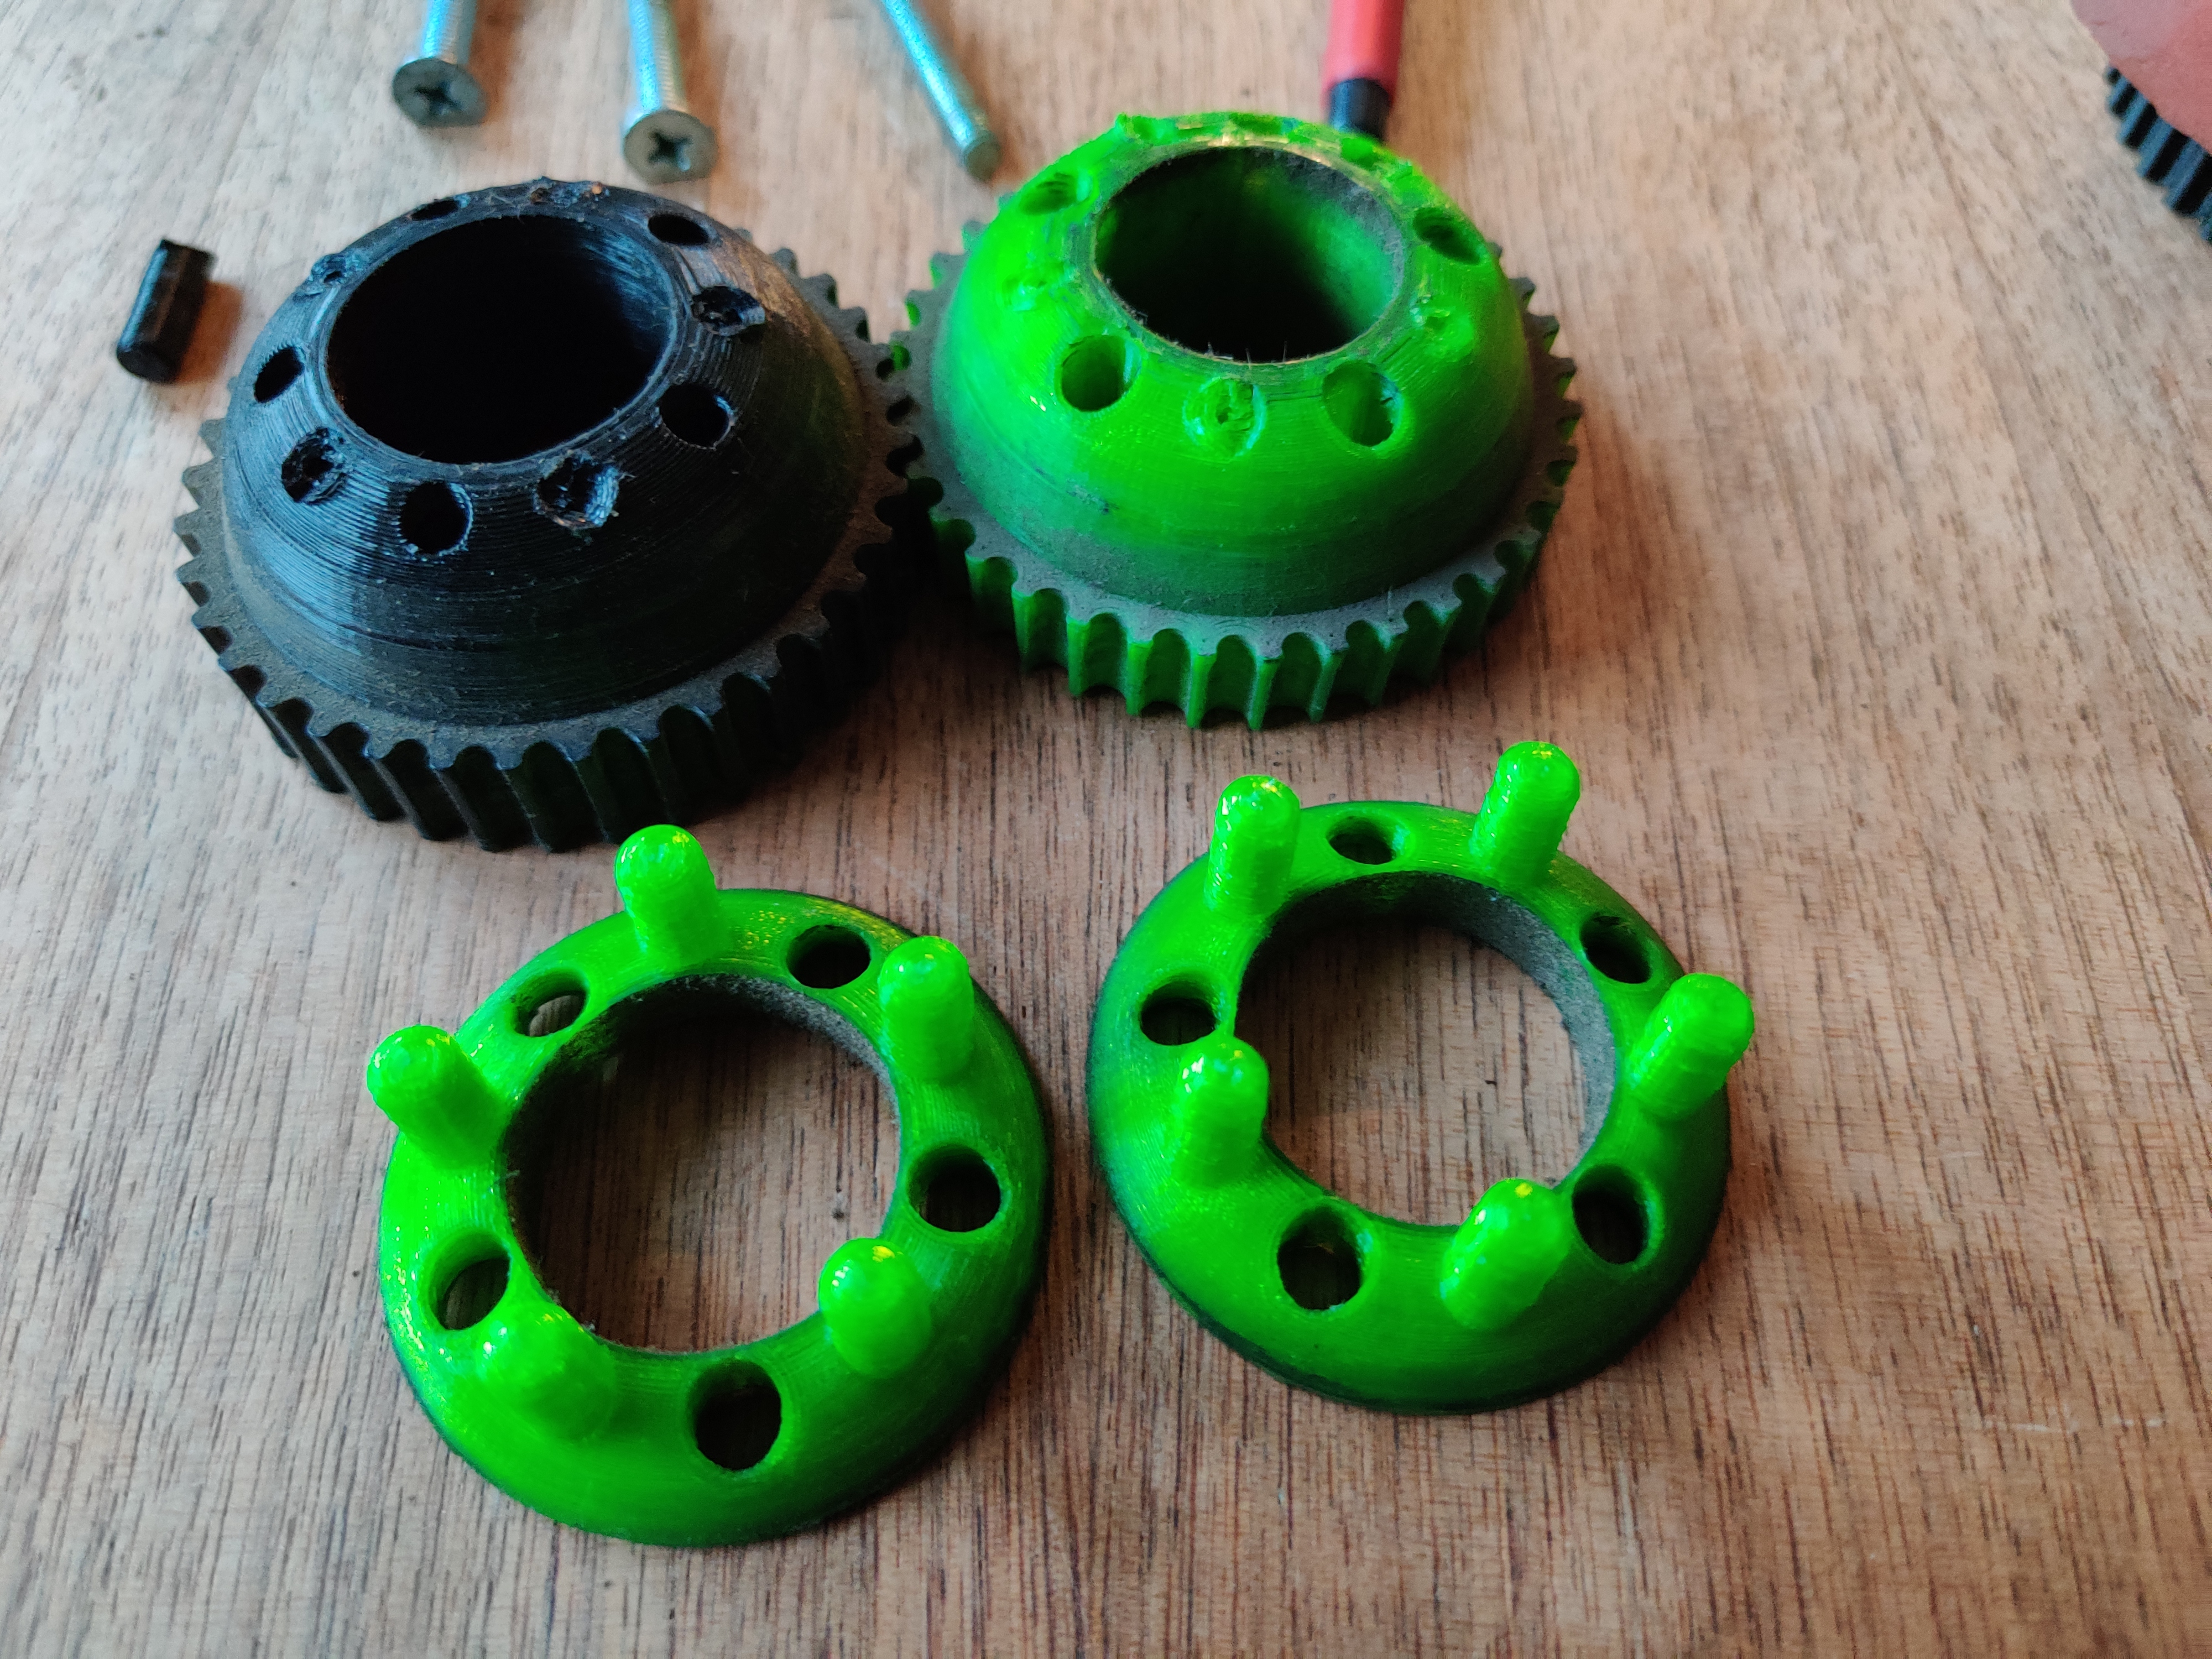
\includegraphics[width=.49\textwidth]{Footage/Pictures/Wheel pulley v1.jpg}
		}
		\caption[Vergleich der gedruckten Zahn- und Konterscheiben vor und nach mehreren Testfahrten]{Links: die finale und zum Zeitpunkt des Verfassens dieses Dokumentes noch verbaute Version. Rechts: der Zustand des ersten funktionalen Prototypes nach etwa \qty{100}{\kilo\metre} Testfahrt. Neben zu erwartender Verschmutzung sei insbesondere auf das Fehlen der Führungsstifte zu achten. Das Zahnprofil und die Komponenten als ganze weisen darüber hinaus jedoch keinerlei Anzeichen von Materialversagen auf.}
		\label{fig:comparison printed parts used unused}
	\end{figure}